\subsection{Introducció a l'estructura de l'aplicació}

    \paragraph{}
    L'aplicació web és relativament simple pel que respecta a la navegació i les diferents seccions que la conformen.

    La figura~\ref{fig:webStructure} mostra l'arbre de continguts accessibles. Cal indicar, que aquesta figura no representa les úniques rutes de navegació existents entre les diferents seccions, sinó un breu mapa del contingut total disponible a través del web i d’on penja cada secció.

    \begin{figure}[h]
        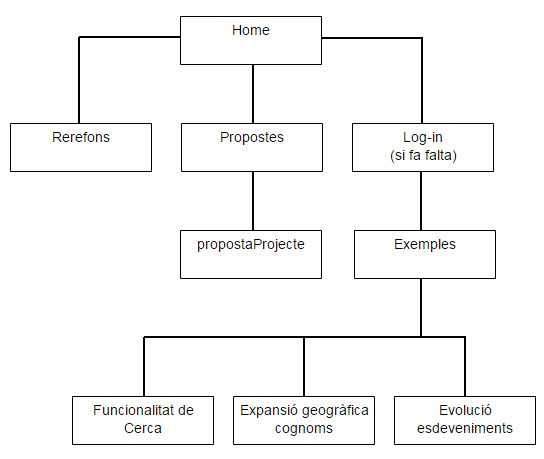
\includegraphics[scale=0.6]{10/01_estructuraWeb}
        \centering
        \caption{Diferents seccions de l'aplicació web}\label{fig:webStructure}
    \end{figure}

    Més endavant, s’explicarà més en detall en què consisteix cada una de les pàgines o seccions de la nostra aplicació web, però primer volem presentar l'estructura general o esquelet, que segueixen gairebé totes les pàgines del nostre web.

    La figura~\ref{fig:pageStructure} mostra l'esquema bàsic sobre el qual les pàgines són construïdes. Aquest pot ser descrit o desglossat en les següents seccions:

    \begin{enumerate}
        \item \textbf{Barra de navegació:} Permet desplaçar-se per les diferents seccions principals.
        \item \textbf{Capçalera de secció:} Conté el títol i subtítol de la pàgina sobre impressionat a una imatge relacionada.
        \item \textbf{Contingut principal:} El contingut principal i únic d'aquesta pàgina.
        \item \textbf{Footer:} Peu de pàgina. Inclou informació sobre el codi font del projecte, la llicència i la facultat d'informàtica de Barcelona.
    \end{enumerate}

    \begin{figure}[h]
        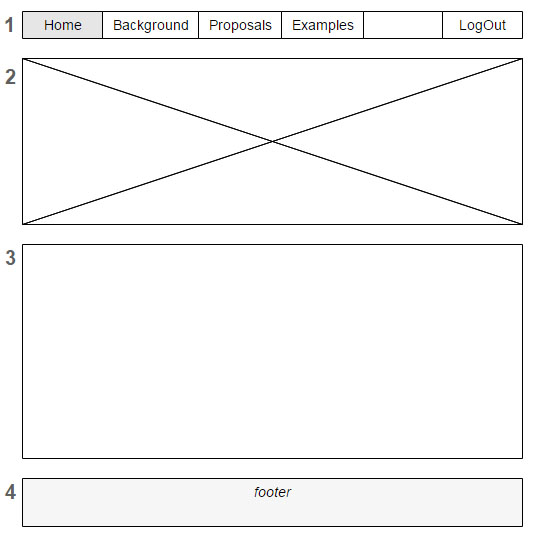
\includegraphics[scale=0.6]{10/02_pagesStructure}
        \centering
        \caption{Esquema bàsic de les pàgines implementades en el domini web}\label{fig:pageStructure}
    \end{figure}

    Convidem des de la memòria, als usuaris de l'aplicació web, a redimensionar la finestra web per tal d'observar com els continguts de cada pàgina s’adapten al dispositiu que els mostra.

    A continuació descriurem el contingut de cada secció o apartat que conforma la nostra aplicació web.
